\subsection{Задача 1}

На следующем графике показана зависимость диаметра текущего бруса от номера итерации (график сужения):

\begin{figure}[H]
	\begin{center}
		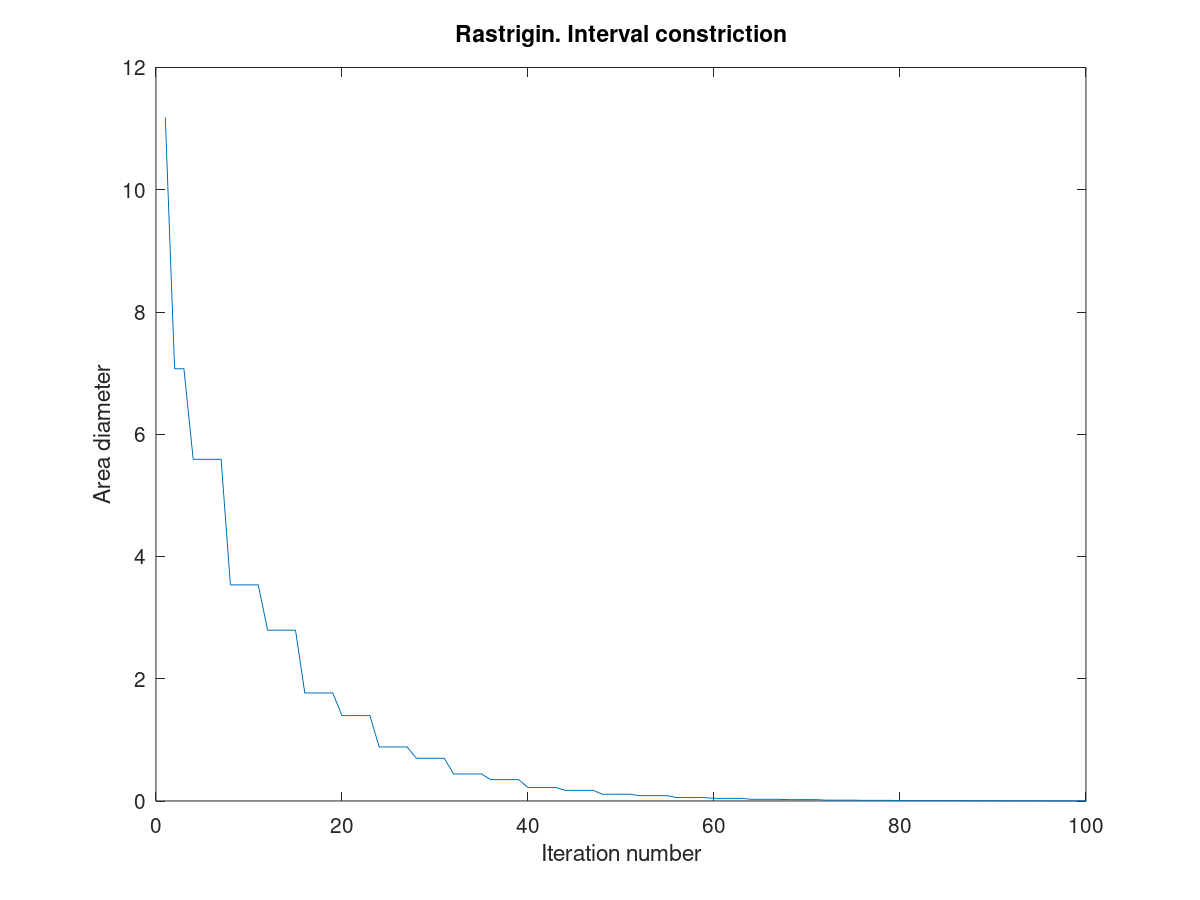
\includegraphics[scale=0.25]{rastrigin}
		\label{pic:rasstrigin_constriction}
		\caption{Функция Растригина. Зависимость диаметра от номера итерации}
	\end{center}
\end{figure}

Для решения данной задачи в функцию GlobOpt0 была добавлена возможность сохранять список диаметров брусов. Кроме того, для удобства использования в GlobOpt0 передаётся указатель на целевую минимизируемую функцию.

На данном рисунке показана траектория центров бруса:

\begin{figure}[H]
	\begin{center}
		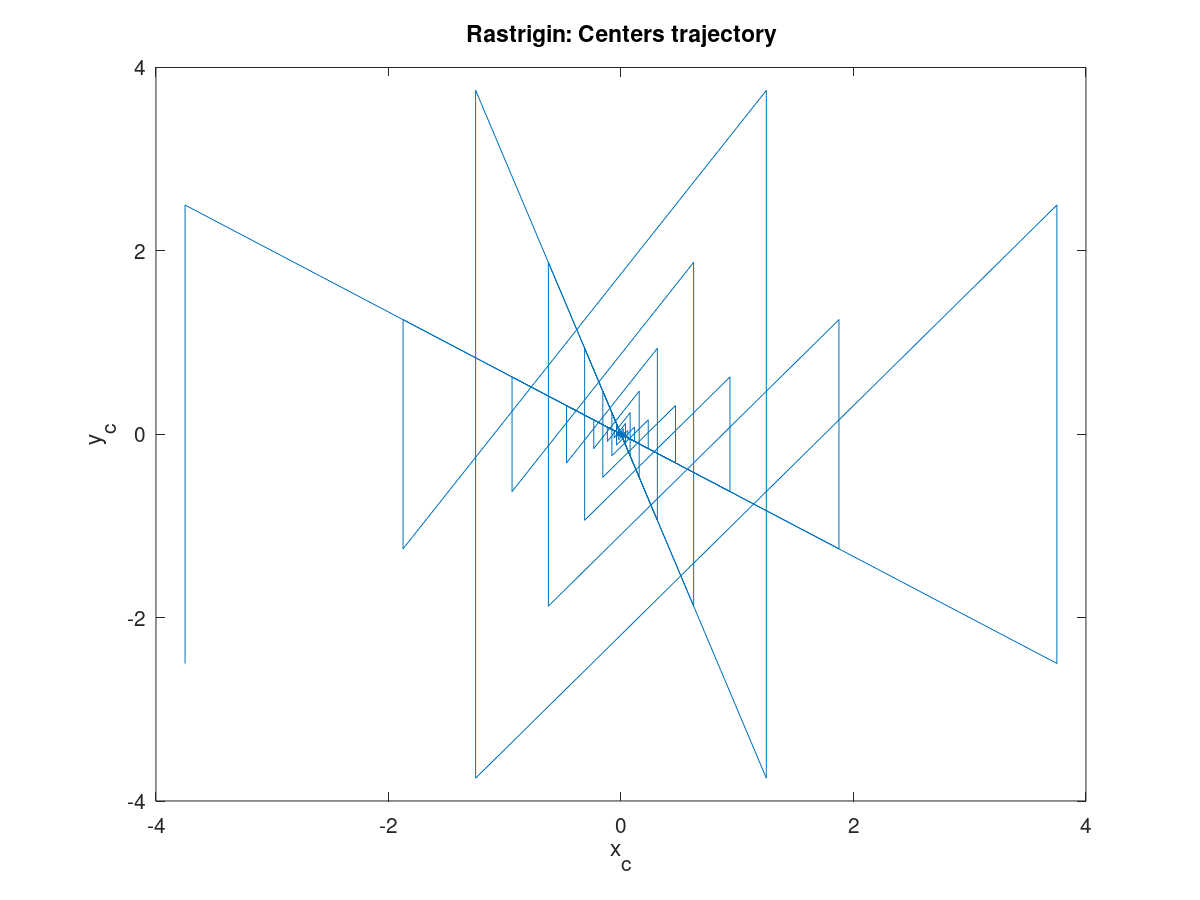
\includegraphics[scale=0.25]{rastrigin_traj}
		\label{pic:rastrigin_traj}
		\caption{Функция Растригина. Траектория центров брусов}
	\end{center}
\end{figure}

\subsection{Задача 2}
На следующем графике показана зависимость расстояния от текущего решения до истинного от номера итерации в полулогарифмических координатах (график сходимости):

\begin{figure}[H]
	\begin{center}
		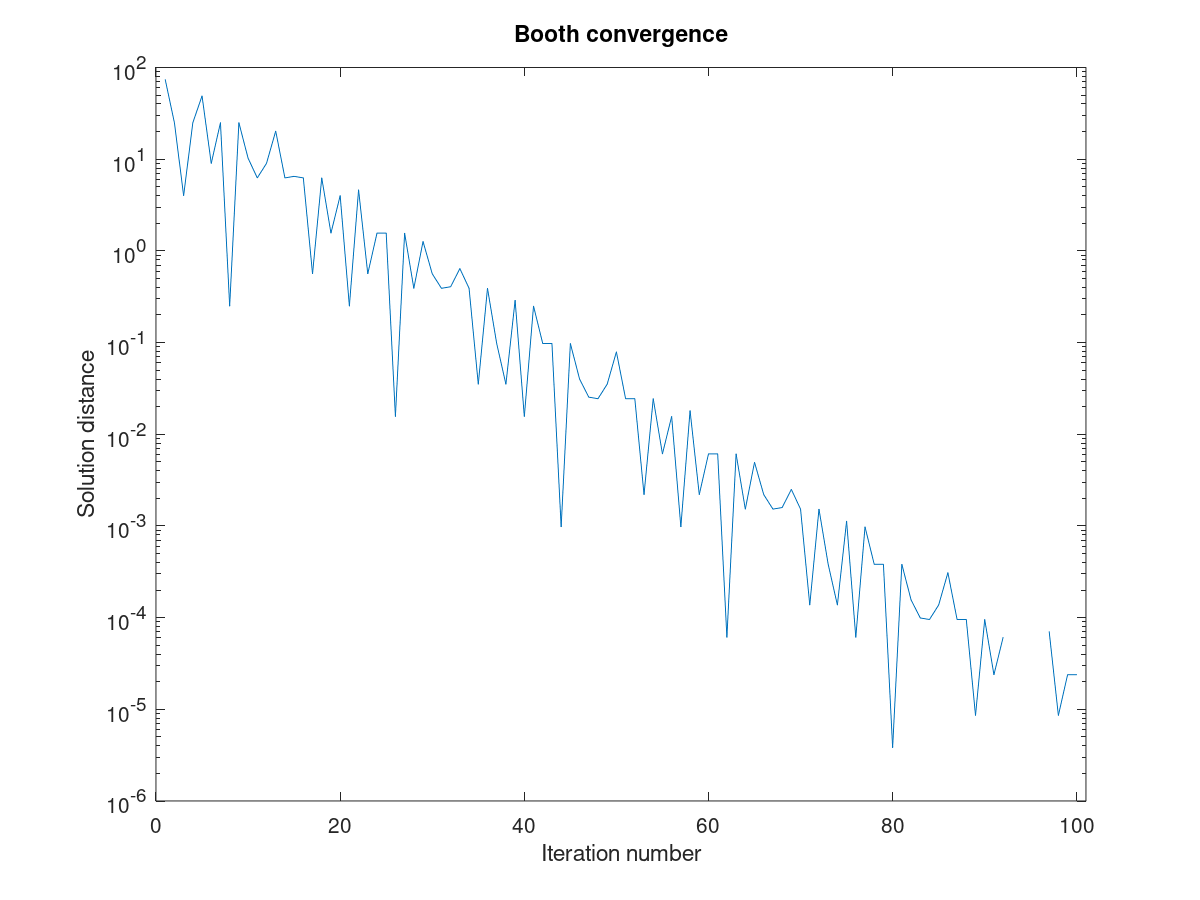
\includegraphics[scale=0.25]{booth_conv}
		\label{pic:booth_conv}
		\caption{Функция Бута. График сходимости}
	\end{center}
\end{figure}

Также в ходе написания обсуждения был построен аналогичны график для функции Растригина:

\begin{figure}[H]
	\begin{center}
		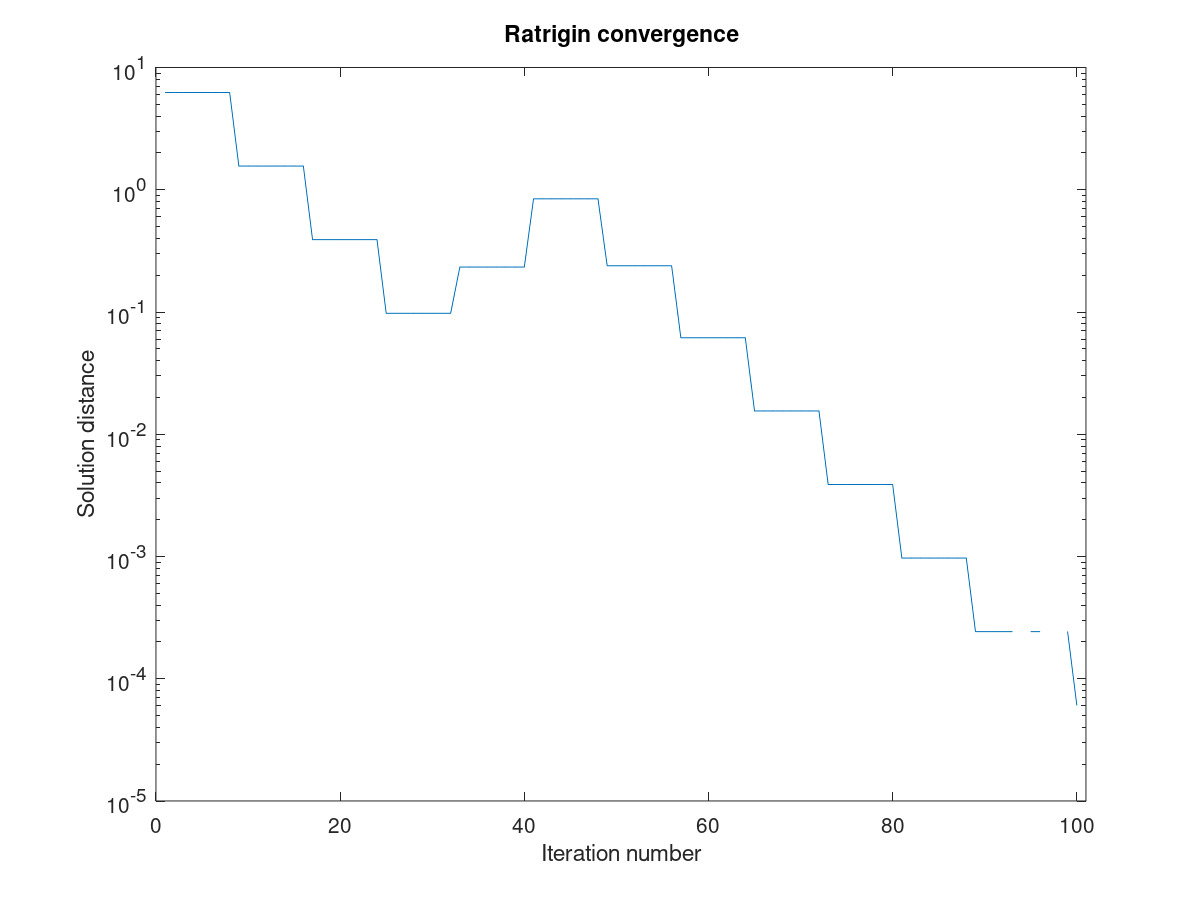
\includegraphics[scale=0.25]{rastrigin_conv}
		\label{pic:rastrigin_conv}
		\caption{Функция Растригина. График сходимости}
	\end{center}
\end{figure}

На данном рисунке показана траектория центров бруса и линии уровня функции Бута:

\begin{figure}[H]
	\begin{center}
		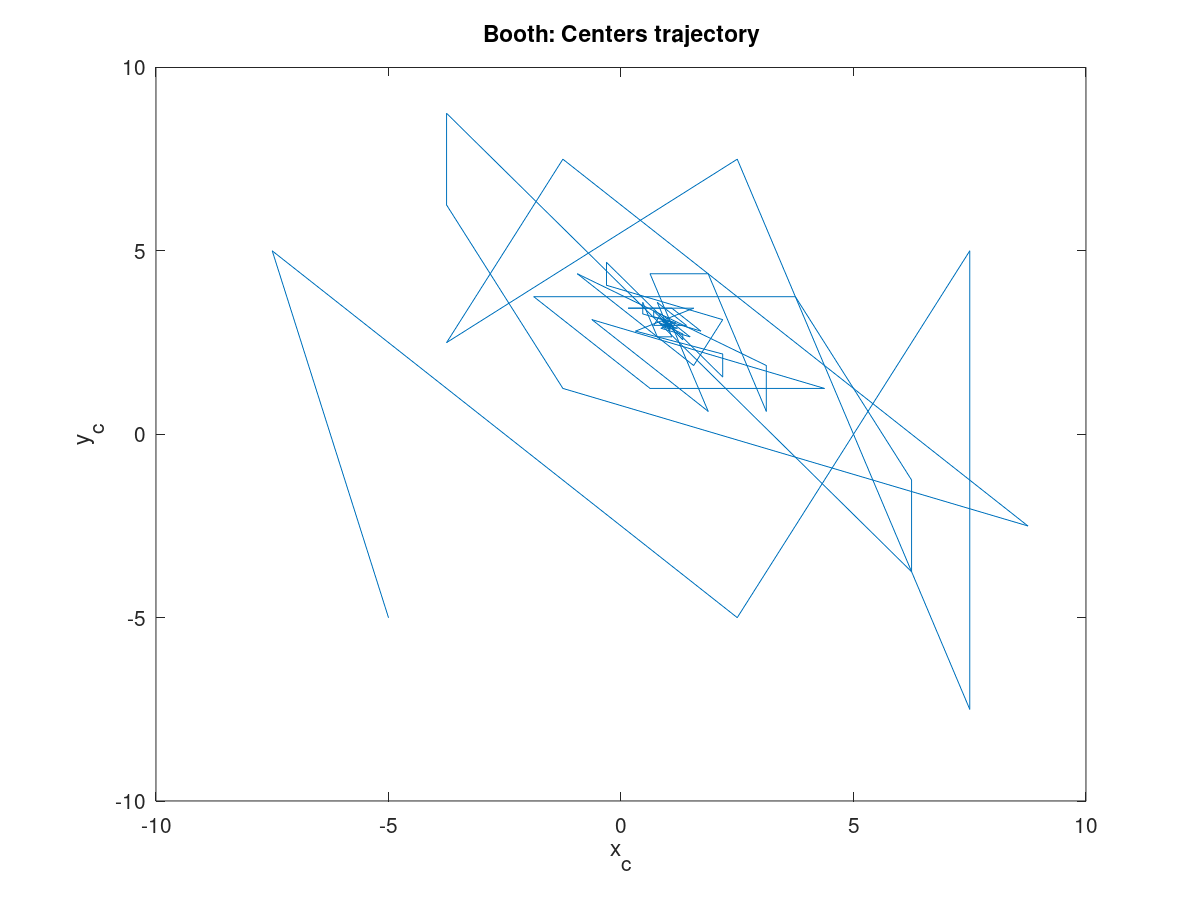
\includegraphics[scale=0.25]{booth_traj}
		\label{pic:booth_traj}
		\caption{Функция Бута. Траектория центров брусов. Линии уровня}
	\end{center}
\end{figure}
